\section{Coexistence Scenarios}

The previous section investigated the borders where stable cycles disappear.
We can see that parameter regions where only one stable cycle exists (``Type A'') can overlap.
For example, the upper border where the cycle $\Cycle{\A^5\B^3\C^5\D^3}$ disappears, marked blue in \Cref{fig:final.regions.E.halved}, is above the lower border where the stable cycle $\Cycle{\A^4\B^3\C^4\D^3}$ disappears, marked red.
This means that there is a coexistence of the cycles in the overlapping parameter region, marked with the point $M$.
This section will take a look at all possible coexistence scenarios of cycles starting with the simplest case, a single ``Type A'' parameter region.

\begin{figure}
    \centering
    \begin{subfigure}{0.4\textwidth}
        \centering
        \includegraphics[width=\textwidth]{60_MinimalRepr/2D_Regions_E/result.png}
        \caption{Showing $E_{16}$}
        \label{fig:final.regions.E.halved}
    \end{subfigure}
    \begin{subfigure}{0.4\textwidth}
        \centering
        \includegraphics[width=\textwidth]{60_MinimalRepr/2D_Regions_F/result.png}
        \caption{Showing $F_{16}$}
        \label{fig:final.regions.F.halved}
    \end{subfigure}
    \caption{2D Period Regions of Halved Final Model Showing a ``Type A'' and a ``Type B'' Region}
\end{figure}

\subsection{Only One ``Type A'' Parameter Region}

As mentioned above, the simplest case of coexistence in this model is the existence of a stable cycle of a ``Type A'' parameter region on its own.
A point where this is the case is the point $L$ in \Cref{fig:final.regions.E.halved}.
Here there is only one stable cycle, $\Cycle{\A^5\B^3\C^5\D^3}$.

\subsection{Two ``Type A'' Parameter Regions Overlapping}
\label{sec:minrep.coex.AA}

``Type A'' parameter regions can overlap with one another.
This can happen in four different ways.
Assuming the stable cycle of the parameter region in the middle is $\Cycle{\A^x\B^y\C^x\D^y}$, it can overlap with parameter regions, where either one of the following cycles is stable
\begin{enumerate*}
    \item $\Cycle{\A^{x-1}\B^y\C^{x-1}\D^y}$,
    \item $\Cycle{\A^x\B^{y+1}\C^x\D^{y+1}}$,
    \item $\Cycle{\A^{x+1}\B^y\C^{x+1}\D^y}$, and
    \item $\Cycle{\A^x\B^{y-1}\C^x\D^{y-1}}$.
\end{enumerate*}
For the concrete case pictured in \Cref{fig:final.regions.E.halved}, this results in the following parameter regions
\begin{enumerate}
    \item $\P_{\A^5\B^3\C^5\D^3, \A^4\B^3\C^4\D^3}$ marked with $M$,
    \item $\P_{\A^5\B^3\C^5\D^3, \A^5\B^4\C^5\D^4}$ marked with $N$,
    \item $\P_{\A^5\B^3\C^5\D^3, \A^6\B^3\C^6\D^3}$ marked with $O$, and
    \item $\P_{\A^5\B^3\C^5\D^3, \A^5\B^2\C^5\D^2}$ marked with $P$.
\end{enumerate}

\begin{figure}
    \centering
    \begin{subfigure}{0.4\textwidth}
        \includegraphics[width=\textwidth]{60_MinimalRepr/Cobweb_M/result.png}
        \caption{At Point $M$}
        \label{fig:minrep.cobweb.M}
    \end{subfigure}
    \begin{subfigure}{0.4\textwidth}
        \includegraphics[width=\textwidth]{60_MinimalRepr/Cobweb_N/result.png}
        \caption{At Point $N$}
        \label{fig:minrep.cobweb.N}
    \end{subfigure}
    \begin{subfigure}{0.4\textwidth}
        \includegraphics[width=\textwidth]{60_MinimalRepr/Cobweb_O/result.png}
        \caption{At Point $O$}
        \label{fig:minrep.cobweb.O}
    \end{subfigure}
    \begin{subfigure}{0.4\textwidth}
        \includegraphics[width=\textwidth]{60_MinimalRepr/Cobweb_P/result.png}
        \caption{At Point $P$}
        \label{fig:minrep.cobweb.P}
    \end{subfigure}
    \caption{Cobwebs for Scenario of Two Overlapping ``Type A'' Parameter Regions}
\end{figure}

\subsection{Only one ``Type B'' Parameter Region}

Another very simple case is when a ``Type B'' parameter region does not overlap with any other region.
In this case, there are two coexisting stable cycles as discussed before in \Cref{sec:og.dynamics}.
Here the cycles are asymmetrical, if one of the cycles is $\Cycle{\A^x\B^y\C^{x-1}\D^{y+1}}$, the other cycle is $\Cycle{\A^{x-1}\B^{y+1}\C^x\D^y}$.
In the concrete case marked in \Cref{fig:final.regions.F.halved} as point $Q$, these cycles are $\Cycle{\A^5\B^3\C^4\D^4}$ and $\Cycle{\A^4\B^4\C^5\D^3}$.

\subsection{One ``Type B'' and One ``Type A'' Parameter Region Overlapping}
\label{sec:minrep.coex.BA}

We can see in \Cref{fig:final.regions.F.halved}, that this ``Type B'' parameter region can overlap with ``Type A'' parameter regions.
This can also happen in four different ways, as was the case with ``Type A'' parameter regions overlapping with one another (described in \Cref{sec:minrep.coex.AA}).
Assuming the stable cycles of the parameter region in the middle are $\Cycle{\A^x\B^y\C^{x-1}\D^{y+1}}$ and $\Cycle{\A^{x-1}\B^{y+1}\C^x\D^y}$, it can overlap with parameter regions, where either one of the following cycles is stable
\begin{enumerate*}
    \item $\Cycle{\A^{x-1}\B^{y+1}\C^{x-1}\D^{y+1}}$,
    \item $\Cycle{\A^x\B^{y+1}\C^x\D^{y+1}}$,
    \item $\Cycle{\A^x\B^y\C^x\D^y}$, and
    \item $\Cycle{\A^{x-1}\B^y\C^{x-1}\D^y}$.
\end{enumerate*}
So in these cases, there will be three coexisting stable cycles.
For the concrete case pictured in \Cref{fig:final.regions.F.halved}, this results in the following parameter regions
\begin{enumerate}
    \item $\P_{\A^5\B^3\C^4\D^4, \A^4\B^4\C^5\D^3, \A^4\B^4\C^4\D^4}$ marked with $R$,
    \item $\P_{\A^5\B^3\C^4\D^4, \A^4\B^4\C^5\D^3, \A^5\B^4\C^5\D^4}$ marked with $S$,
    \item $\P_{\A^5\B^3\C^4\D^4, \A^4\B^4\C^5\D^3, \A^5\B^3\C^5\D^3}$ marked with $T$, and
    \item $\P_{\A^5\B^3\C^4\D^4, \A^4\B^4\C^5\D^3, \A^4\B^3\C^4\D^3}$ marked with $U$.
\end{enumerate}

\begin{figure}
    \centering
    \begin{subfigure}{0.4\textwidth}
        \includegraphics[width=\textwidth]{60_MinimalRepr/Cobweb_R/result.png}
        \caption{At Point $R$}
        \label{fig:minrep.cobweb.R}
    \end{subfigure}
    \begin{subfigure}{0.4\textwidth}
        \includegraphics[width=\textwidth]{60_MinimalRepr/Cobweb_S/result.png}
        \caption{At Point $S$}
        \label{fig:minrep.cobweb.S}
    \end{subfigure}
    \begin{subfigure}{0.4\textwidth}
        \includegraphics[width=\textwidth]{60_MinimalRepr/Cobweb_T/result.png}
        \caption{At Point $T$}
        \label{fig:minrep.cobweb.T}
    \end{subfigure}
    \begin{subfigure}{0.4\textwidth}
        \includegraphics[width=\textwidth]{60_MinimalRepr/Cobweb_U/result.png}
        \caption{At Point $U$}
        \label{fig:minrep.cobweb.U}
    \end{subfigure}
    \caption{Cobwebs for Scenario of a ``Type B'' and a ``Type B'' Parameter Region Overlapping}
\end{figure}

\subsection{One ``Type B'' and Two ``Type A'' Parameter Regions Overlapping}

When looking closer at \Cref{fig:final.regions.F.halved}, one can see that the parameter regions described in the previous \Cref{sec:minrep.coex.BA} also overlap with one another.
This results in parameter regions where there are two stable cycles from a ``Type B'' parameter region and two stable cycles, each from one ``Type A'' parameter region, coexisting.
So there are four parameter regions for every ``Type B'' parameter region, where four stable cycles are coexisting.
For the stable cycles $\Cycle{\A^x\B^y\C^{x-1}\D^{y+1}}$ and $\Cycle{\A^{x-1}\B^{y+1}\C^x\D^y}$ in the ``Type B'' parameter region, the cycles they will coexist with are pairs of the cycles discussed in \Cref{sec:minrep.coex.BA}.
They are
\begin{enumerate*}
    \item $\Cycle{\A^{x-1}\B^{y+1}\C^{x-1}\D^{y+1}}$ and $\Cycle{\A^x\B^{y+1}\C^x\D^{y+1}}$,
    \item $\Cycle{\A^x\B^{y+1}\C^x\D^{y+1}}$ and $\Cycle{\A^x\B^y\C^x\D^y}$,
    \item $\Cycle{\A^x\B^y\C^x\D^y}$ and $\Cycle{\A^{x-1}\B^y\C^{x-1}\D^y}$, and
    \item $\Cycle{\A^{x-1}\B^y\C^{x-1}\D^y}$ and $\Cycle{\A^{x-1}\B^{y+1}\C^{x-1}\D^{y+1}}$.
\end{enumerate*}
For the concrete case pictured in \Cref{fig:final.regions.F.halved}, this results in the following parameter regions
\begin{enumerate}
    \item $\P_{\A^5\B^3\C^4\D^4, \A^4\B^4\C^5\D^3, \A^4\B^4\C^4\D^4, \A^5\B^4\C^5\D^4}$ marked with $V$,
    \item $\P_{\A^5\B^3\C^4\D^4, \A^4\B^4\C^5\D^3, \A^5\B^4\C^5\D^4, \A^5\B^3\C^5\D^3}$ marked with $W$,
    \item $\P_{\A^5\B^3\C^4\D^4, \A^4\B^4\C^5\D^3, \A^5\B^3\C^5\D^3, \A^4\B^3\C^4\D^3}$ marked with $X$, and
    \item $\P_{\A^5\B^3\C^4\D^4, \A^4\B^4\C^5\D^3, \A^4\B^3\C^4\D^3, \A^4\B^4\C^4\D^4}$ marked with $Y$.
\end{enumerate}

\begin{figure}
    \centering
    \begin{subfigure}{0.4\textwidth}
        \includegraphics[width=\textwidth]{60_MinimalRepr/Cobweb_V/result.png}
        \caption{At Point $V$}
        \label{fig:minrep.cobweb.V}
    \end{subfigure}
    \begin{subfigure}{0.4\textwidth}
        \includegraphics[width=\textwidth]{60_MinimalRepr/Cobweb_W/result.png}
        \caption{At Point $W$}
        \label{fig:minrep.cobweb.W}
    \end{subfigure}
    \begin{subfigure}{0.4\textwidth}
        \includegraphics[width=\textwidth]{60_MinimalRepr/Cobweb_X/result.png}
        \caption{At Point $X$}
        \label{fig:minrep.cobweb.X}
    \end{subfigure}
    \begin{subfigure}{0.4\textwidth}
        \includegraphics[width=\textwidth]{60_MinimalRepr/Cobweb_Y/Manual/result.png}
        \caption{At Point $Y$}
        \label{fig:minrep.cobweb.Y}
    \end{subfigure}
    \caption{Cobwebs for Scenario of a ``Type B'' Parameter Region and Two ``Type A'' Parameter Regions Overlapping}
\end{figure}
